The era of Big Data is upon us bringing with it a range of new challenges "Without big data, you are blind and deaf and in the middle of a freeway."\cite{moore} . The importance which accompany these challenges encouraged the formulation of new approaches for cleaning, processing and using enormous amounts of data. (Section \ref{bigdata})

Data is being collated and stored every second of every day and the value of doing so has never been greater. Billion dollar companies such as Google and Amazon dominate the market in data collection and pride themselves in knowing everything about everything. Former CEO of Google, Eric Schmidt famously said in 2010 "We know where you are. We know where you've been. We can more or less know what you're thinking..." \cite{schmidt}. Thus the power of data collection has led to the development of a range of technologies designed to meet the needs of Big Data.

The purpose of the following research, by way of investigation, is to deliver an insightful examination of a subset of new technologies which deliver high performance querying of large datasets. The ultimate aim of the research is to gain an understanding of these technologies and achieve a level of mastery which permits a thorough scrutiny of their application to Big Data.

There are a number of different indexing solutions available however for the means of this project to encapsulate a comprehensive examination a focus will be on leading NoSQL solutions, modern search and analytics engines and for comparative reasons a conventional relational database management system. The following technologies which will be used for the project: 

\begin{itemize}
\item MongoDB (Section \ref{mongo})
\item Neo4j (Section \ref{neo})
\item Apache Cassandra (Section \ref{cassandra})
\item MySQL (Section \ref{mysql})
\end{itemize}

\section{Objectives}\label{objectives}
The three key objectives and main intended outcomes for the project are:
\begin{enumerate}
\item Investigate the strengths and weaknesses of the functionality each technology provides.
\item Compare and contrast the analytical capabilities of each technology by way querying prototype models.
\item Conduct a comparative analysis to investigate the scalability of each technology.
\end{enumerate}

\section{Motivation}
My interest in the field of data science stems from university modules I have undertaken as part of my BSc Computer Science degree such as 'Database Management Systems' and a course I am currently studying 'Data Mining and Machine Learning'. The material involved in these courses gave me an insight in to the field of data science and provided me with the opportunity to get a hands on feel for the manipulation, cleansing and processing of a variety of real life data sets and database systems.

Whilst studying for my degree I have undertaken modules which have stipulated a working knowledge of MySQL as a prerequisite therefore my comprehension of MySQL is proficient. One of the main attractions to undertaking this project was to be given the opportunity to learn about a number of next generation database management systems. It was important for me to undertake a project in which I will be able to apply my learning and findings to progress in a career path within the data science field.

\section{Definitions}
The data source being used in this document comes from the biological field and therefore relies on an apprehension of basic concepts and terms. The below table of definitions provides an overview in to some of these terms to develop a level of understanding and aid the reader of the document. The table also includes the definitions of generally unknown terms and phrases which will be discussed throughout this project.

\begin{center}
    \begin{tabular}{ |p{0.3\linewidth} | p{0.7\linewidth} |}
    \hline
    \textbf{Term} & \textbf{Definition} \\ \hline
    Edinburgh Mouse Atlas Project (EMAP) & The combined research projects of Dr Duncan Davidson and Prof Richard Baldock. \\ \hline
    EMAP \textbf{anatomy} & A freely available, structured, \textbf{stage specific} list of 13,000+ terms that describe visible anatomical structures in the developing mouse embryo. \\ \hline
    Edinburgh Mouse Atlas Project Abstract (EMAPA) & A refined and algorithmically developed \textbf{non-stage specific} anatomical ontology representation of the EMAP anatomy. \\ \hline
    Edinburgh Mouse Atlas of Gene Expression (EMAGE) & A database of in situ gene expression data in the developing mouse embryo  \\ \hline
    Theiler Stage (TS) & Each stages defines the development of a mouse embryo by a set of organism structure criteria. \\ \hline
    Not only SQL (NoSQL) & A non-relational database environment which is useful for very large sets of distributed data. Allows rapid, ad-hoc organisation and analysis of extremely high-volume, disparate data types. \\ \hline
        Ontology & Refers to the science of describing the kinds of entities in the world and how they are related. \\ \hline
            Web Ontology Language (OWL) & A language representation standard for designing and authoring Web ontologies produced from the World Wide Web Consortium W3C. \\ \hline
          OBO & A flat file format ontology representation language \\ \hline
    \end{tabular}
\end{center}

\section{Project Plan}
The below gantt chart illustrates the time scale in which deadlines and deliverables will be met throughout the project.
\begin{sidewaysfigure}[ht]
    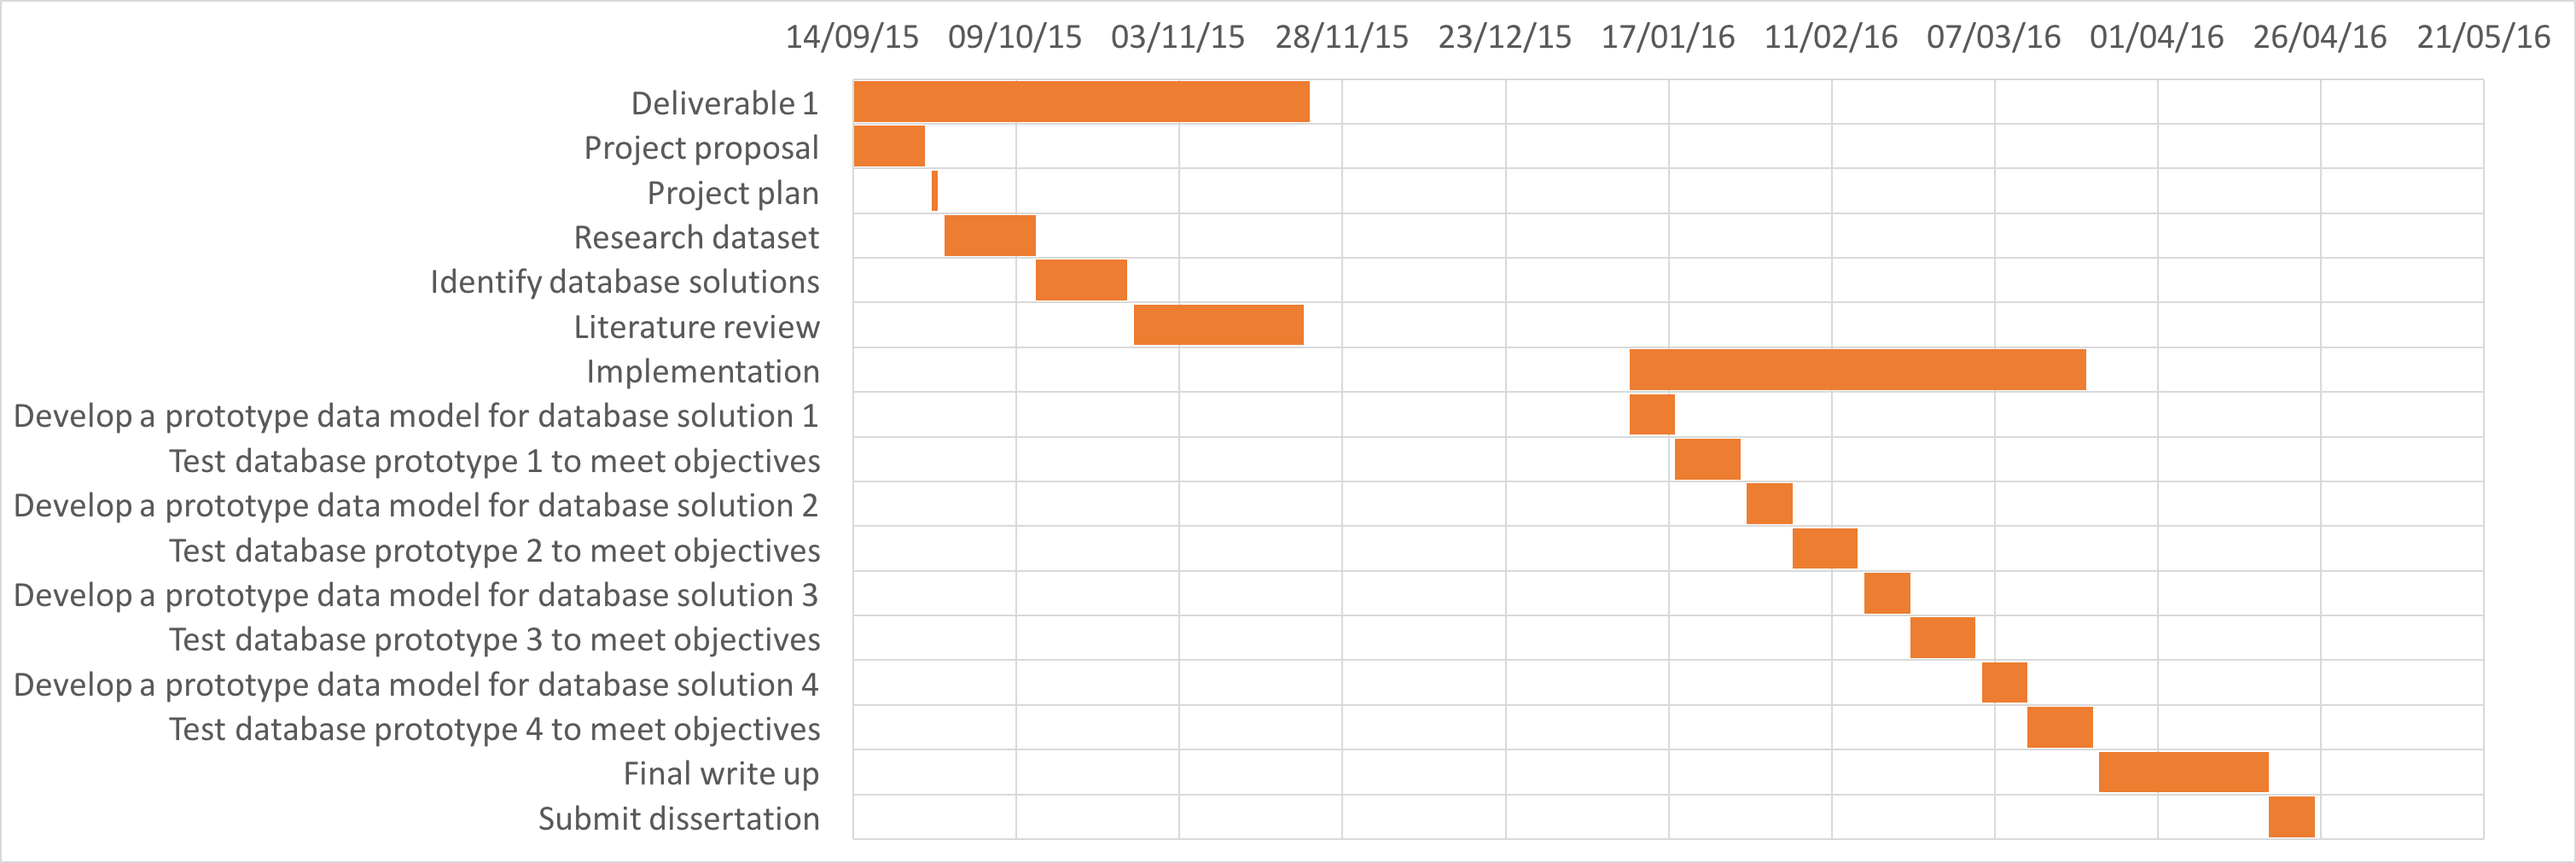
\includegraphics[height=15cm, width = 1\linewidth]{images/gantt}
\end{sidewaysfigure}
